\documentclass[12pt,a4paper,titlepage]{article}
\usepackage[latin1]{inputenc}
\usepackage{amsmath}
\usepackage{amsfonts}
\usepackage{amssymb}
\usepackage{makeidx}
\usepackage{graphicx}
\usepackage{subcaption}

\makeatletter
\setlength{\@fptop}{0pt}
\makeatother

\oddsidemargin 1cm
\evensidemargin 1cm
\textwidth 15cm
\topmargin -1.25cm
\textheight 24.37cm

\renewcommand{\listfigurename}{Figures}
\renewcommand{\listtablename}{Tables}

\begin{document}	
	\begin{titlepage}
		\begin{figure}
			
\includegraphics[width=.6\linewidth]{images/logoWWU}
		\end{figure}
		\vspace*{2cm}
		\begin{center}
			Title:\\			
			\textbf{Application of Data Analytics in Failure Pattern Recognition}
			
			\vspace*{3cm}
			\textbf{Seminar Thesis}\\			
			In the context of the seminar ``Application of Data Analytics in Spare Parts Supply Chain Management''\\
			at the Chair for Information Systems and Supply Chain Management
		\end{center}
		\vspace*{1.5cm}
		\begin{tabbing}
			\hspace*{4cm}\= \kill
			Supervisors:			\> Dr.-Ing.Christian Grimme\\
									\> Dipl.-Inf. Jakob Bossek\\
									\> Carolin Wagner MScIS\\
			\\
			Presented by:			\> Alexander Anokhin\\
									\> Busso-Peus-Str. 14\\
									\> Muenster 48149\\
									\> Germany\\
									\> +4917675615943\\
									\> a\_anok01@uni-muenster.de\\
									\\
									\> Joshua Peter Handali\\
									\> Street\\
									\> Muenster zip-code\\
									\> Germany\\
									\> Mobile Phone\\
									\> j\_hand01@uni-muenster.de\\
			\\
			Date of submission: 	\> \today\\
		\end{tabbing}
	\end{titlepage}	
	
	\pagenumbering{gobble}
	\tableofcontents
	\newpage	
	
	\pagenumbering{Roman} 
	\setcounter{page}{1}
	\clearpage
	
	\addcontentsline{toc}{section}{Figures}
	\listoffigures
	\newpage
		
	\addcontentsline{toc}{section}{Tables}
	\listoftables
	\newpage
	
	\section*{Abbreviations}
	\addcontentsline{toc}{section}{Abbreviations}
	\begin{tabbing}
		\hspace*{3cm}\= \kill
		ANN				\> Artificial Neural Networks\\
		ANOVA RBF		\> ANOVA Radial Basis Function\\ 
		CART			\> Classification and Regression Trees\\
		ICA				\> Independent Component Analysis\\
		PCA				\> Principal Component Analysis\\
		SVM				\> Support Vector Machine\\		
	\end{tabbing}
	\newpage
	
	\pagenumbering{arabic} 
	\setcounter{page}{1}
	\section*{Introduction 1 page}
	\label{introduction}
	\addcontentsline{toc}{section}{Introduction}
	Support vector machine (SVM) is a relatively new computational learning method based on the statistical learning theory. Exhaustive overviews of SVM applicability in pattern recognition \cite{Lee2002} and fault diagnosis \cite{Widodo20072560} clearly show that SVM is a versatile and efficient technique for such problems. The concept of SVM is based on Vapnik-Chervonenkis theory \cite{cortes1995support, vapnik1995nature} that recently emerged as a general mathematical framework for estimating (learning) dependencies from finite samples \cite[p. 2561]{Widodo20072560}. The idea of SVM is to separate feature space by constructing linear boundaries between two classes. Moreover initial feature space can be enlarged with help of kernel transformations. 
		
	SVM approach is not only theoretically well-founded, but also superior in practice. Recent surveys show that tuned SVM classifiers has become more efficient in pattern recognition than other methods: Artificial Neural Networks (ANN) \cite{Deng20116007, Jodas2013240, Kamruzzaman2006, pan2012parkinson, Shao201278} and Classification and Regression Trees (CART) \cite{marnerides2015fault, Shao201278}. In addition, SVMs have one significant advantage compared to conventional methods of pattern recognition such as ANNs. These methods straggle to solve problems with a small number of samples. For the reason that it is hard to obtain sufficient fault samples in practice, SVM is introduced into machines fault diagnosis due to its high accuracy and good generalization for a smaller number of samples \cite[p. 2562]{Widodo20072560}. 
	
	\section{Problem Description}
	\subsection{Research Methodology}
	Aim of analysis is to build a classifier, based on initially collected data, to detect failures. Such a diagnosis can highly benefit company in real life, since failures identified at early stage future costly faults possibly prevented. The aim defines a number of research questions. First of all, it is unclear how the initially proposed data can be properly preprocessed. Moreover, since classes are possible unbalanced another question is how they can be balanced and should they be balanced at all. Since feature extraction and selection as well as SVM parametrization are highly effect final results it will be also valuable to answer the question about optimal procedure and parameters. Another question is how accuracy and efficiency of a classifier can vary along different settings, for example size of initial sample. 
	
	To accomplish the aim of a study research design was mainly based on optimization and simulation experiments, however literature research was also used in two ways: establish a proper direction of analysis; identify for further use existing methods and approaches. Analysis was conducted with help of R programming language\footnote{http://www.r-project.org/} which was used for statistical computing and graphics.
	
	\subsection{Data Description}
	The initial data is provided by a Brazilian manufacturer. The company produces different kinds of	electric actuators to drive control values. Data are generated in a test environment under normal and overload conditions. Three sensors are installed near the
	gears that are able to record the incurring vibration. The test environment is depicted at Figure \ref{fig:testEnvironment}. Sensor 1 is located in the bearing of the main spindle, Sensor 2 on the motor's bearing and Sensor 3 depicts a built-in torque sensor.
		
	\begin{figure}[h!]
		\centering
		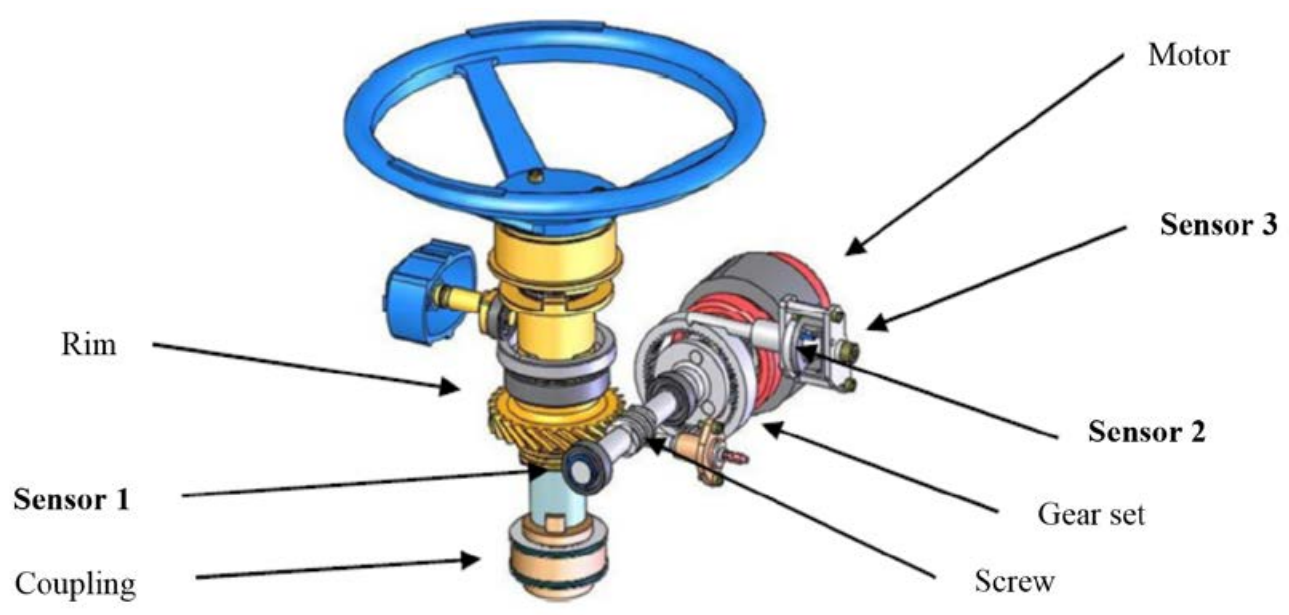
\includegraphics[width=1\linewidth]{images/testEnvironment}
		\label{fig:polinom}
		\caption{Test Environment}
		\label{fig:testEnvironment}
	\end{figure}	  
	
	Tests perform valve aperture actions and are initiated under different conditions. New gears are	considered with and without additional load. In addition, failure data is obtained using worn and broken gears therefore provided data comprises six different settings with three types of failures. For every second is collected 2048 observations of signal. Each cycle lasts about 46-47 seconds. Table \ref{table:generatedData} summarizes generated data.
	
	\begin{table}[h!]
		\centering
		\begin{tabular}{ | l | l | c | c | }
			\hline
			\multicolumn{1}{ | c | }{\textbf{Class}} 
				& \multicolumn{1}{ | c | }{\textbf{Description}}
				& \multicolumn{1}{ | c | }{\textbf{Cycles}} 	
				& \multicolumn{1}{ | c | }{\textbf{Observations}}\\
			\hline
			Normal 1 	& Cycle without load on actuator 			& 25 		& $2398*10^3$\\
			Normal 2 	& Cycle with pressure equal 3.0 bar 		& 25 		& $2572*10^3$\\
			Normal 3 	& Cycle with pressure equal 1.0 bar 		& 25 		& $2392*10^3$\\
			Failure 1 	& Cycle with a worn gear without load 		& 10 		& $930*10^3$\\
			Failure 2 	& Cycle with two worn gears without load 	& 2 		& $195*10^3$\\
			Failure 3 	& Cycle with a broken gear without load 	& 10 		& $946*10^3$\\
			\hline
		\end{tabular}
		\caption{Generated Data} 
		\label{table:generatedData}
	\end{table}
	
	Table \ref{table:generatedData} outlines three important aspects of further analysis. First, provided data are highly unbalanced along classes. The most unbalance case is between Normal 2 and Failure 2 classes. The unbalance ratio here accounts for 75:1000. Second, generated data consist of about 10 millions observations in total which makes computationally impossible to use SVM directly. Third, slightly more emphasis in analysis is putted on comparison of Normal 1 and failure classes since they have been all obtained without load. That is premised in assumption of being able to measure load directly. Since load is measured we can explicitly exclude classes with or without load depending on estimated load. 
	
	\section{Data Preparation}
	\subsection{Data Preprocessing}
	To achieve appropriate performance and classification results data preprocessing step should be done beforehand. The aim of data preprocessing from one side is to reduce the noise in the data and from another side retain as much information as possible. Typically data preprocessing also requires feature extraction step where a set of reasonable features extracted from raw signals.
	
	Generated data contain no missing data or obvious outliers which makes preprocessing step very straightforward. However one issue that affected performance at early stages was discovered. Every cycle has steady states in the beginning and in the end where signal does not change over about one second. That obviously distracts classifier since steady signal can be misclassified as failure which lead to full stop. To avoid such scenarios every second in a cycle was divided into 16 time windows and then for all of them standard deviation was calculated. In result if standard deviation is less than 5\% quantile for a whole cycle then signal during that period of time is considered as stable and related observations removed from further consideration. Figure \ref{fig:signalBehavior} shows this procedure. 
	
	\begin{figure}[h!]
		\centering
		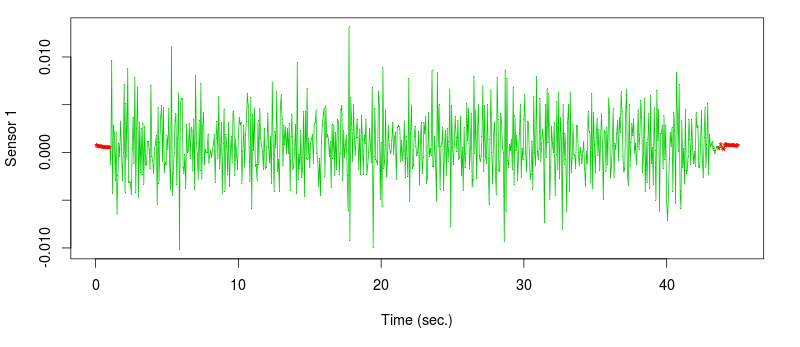
\includegraphics[width=1\linewidth]{images/signalBehavior}
		\caption[Signal Behavior]{Signal Behavior. Red line represents removed observations.}
		\label{fig:signalBehavior}
	\end{figure} 	
		
	Feature extraction step for vibration signal has been already widely explored in literature. Samanta \cite{Samanta2004625} during this step extracted time domain features in order to identify gear faults. That approach was later improved by Soleimani et al. \cite{soleimani2009fault}, vibration was considered not just as time varying but also as a physical signal, thus time domain and frequency domain features were extracted. In this analysis, based on existing research conducted by Soleimani et al. \cite[p. 2]{soleimani2009fault}, vibration signal was considered in time interval of 5 seconds where time domain features were extracted. Table \ref{table:extractedFeatures} presents extracted time domain features.
	
	\begin{table}[h!]
		\centering
		\begin{tabular}{ | l | l | }
			\hline
			\multicolumn{1}{ | c | }{\textbf{Feature}} 
				& \multicolumn{1}{ | c | }{\textbf{Formula}}\\
			\hline
			mean 				& $T_1=\frac{1}{N}\sum_{i=1}^{N}x_i$\\
			standard deviation 	& $T_2=(\frac{1}{N}\sum_{i=1}^{N}(x_i-T_1)^2)^{0.5}$\\
			peak 				& $T_3=max\{x_i\}, i=1,...,N$\\
			root mean square 	& $T_4=(\frac{1}{N}\sum_{i=1}^{N}x_{i}^{2})^{0.5}$\\
			crest factor 		& $T_4=\frac{T_3}{T_4}$\\
			skewness 			& $T_4=\frac{1}{T_{2}^{6}}\sum_{i=1}^{N}(x_{i}-T_1)^3$\\
			kurtosis 			& $T_4=\frac{1}{T_{2}^{8}}\sum_{i=1}^{N}(x_{i}-T_1)^4$\\
			\hline
		\end{tabular}
		\caption{Extracted Time Domain Features} 
		\label{table:extractedFeatures}
	\end{table}	
	
	After data preprocessing and feature extraction size of data was significantly reduced even without feature selection step. Final training sample consist of about 920 observations in total that makes possible to apply SVM in order to classify gear failures. Every observation  consists of 21 features: 7 extracted features for every sensor signal, and  response variable which shows existence of failure.
	
	\subsection{Exploratory Analysis}
	\label{exploratoryAnalysis}
	Another important step in order to build classifier is exploratory analysis. The aim of exploratory analysis is to understand data and check possible underlying assumptions required for analysis. It helps to find incentives for further steps and omit impossible scenarios which saves time and resources. SVM approach is very versatile and does nor require data to follow specific distribution that fact shortened exploratory step. 
	
	Since features were extracted from one signal there is a possibility that some of them are highly correlated and will create unnecessary computational overhead, during the process of training, without improvement of accuracy. It can be clearly seen from Table \ref{table:correlationMatricesOne} that features correlate along one sensor, for example, standard deviation of signal from Sensor 1 functionally determines root mean square for the same signal. In addition, features from different sensors correlate as well. Standard deviation of signal from Sensor 2 correlates with standard deviation of signal but from Sensor 3, which is shown at Table \ref{table:correlationMatricesAll}. These issues highlights the problem of dimensionality reduction which will be explored further in Section \ref{dimensionalityReduction}. 
	
	\begin{table}[h!]
		\begin{subtable}{.5\linewidth}
			\centering
			\begin{tabular}{ | p{.4cm} | p{.4cm} | p{.4cm} | p{.4cm} | p{.4cm} | }
				\hline
				  			& \textbf{1} 	& \textbf{2} 	& \textbf{3} 	& \textbf{4}\\ \hline
				\textbf{1} 	& 1 			& 0 			& .04 			& 0\\ \hline
				\textbf{2} 	&  				& 1 			& .57 			& 1\\ \hline
				\textbf{3} 	&   			&   			& 1 			& .57\\ \hline
				\textbf{4} 	&   			&   			&   			& 1\\ \hline
			\end{tabular}
			\caption{Sensor 1}
			\label{table:correlationMatricesOne}
		\end{subtable}
		\begin{subtable}{.5\linewidth}
			\centering
			\begin{tabular}{ | p{.4cm} | p{.4cm} | p{.4cm} | p{.4cm} | }
				\hline
				  			& \textbf{5}	& \textbf{6} 	& \textbf{7}\\ \hline
				\textbf{5} 	& 1				& .02 			& .4\\ \hline
				\textbf{6} 	&   			& 1 			& .54\\ \hline
				\textbf{7} 	&   			&   			& 1\\ \hline
			\end{tabular}
			\caption{All Sensors}
			\label{table:correlationMatricesAll}
		\end{subtable}
		\caption[Correlation Matrices]{Correlation Matrices. 1 - mean; 2 - standard deviation; 3 - peak; 4 - root mean square; 5, 6, 7 - standard deviations for sensors 1, 2, 3 respectively.}		
	\end{table}
		
	It was outlined before that SVM approach tries to find distinguishing hyperplane between two classes therefore during exploratory analysis it is also valuable to explore how separable observations from different classes. Figure \ref{fig:visualInspection} shows that some classes can be accurately separated using only two features. However it is not the common case for two-dimensional space where some classes have a lot of overlap. For example, classes with normal conditions are hardly separable in two-dimensional space. Of course, using more than two features can lead to accurate separation but it cannot be properly visualize. 
	
	\begin{figure}[!h]
		\begin{subfigure}{.5\textwidth}
			\centering
			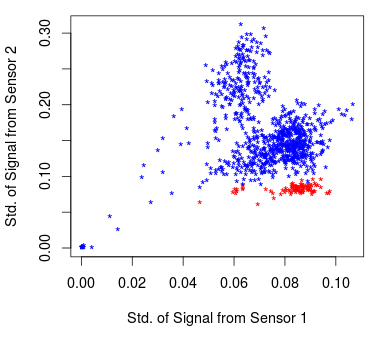
\includegraphics[width=.8\linewidth]{images/visualInspection1}
			\caption{Failure 1}
		\end{subfigure}%
		\begin{subfigure}{.5\textwidth}
			\centering
			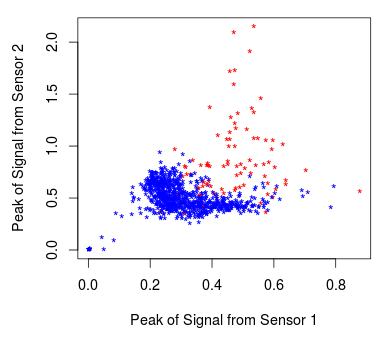
\includegraphics[width=.8\linewidth]{images/visualInspection2}
			\caption{Failure 3}
		\end{subfigure}
			\caption[Separation of Classes]{Separation of Classes. Red stars represent certain failure classes, blue points represent the rest of observations.}
		\label{fig:visualInspection}
	\end{figure}	
	
	Exploratory part here does not pretend to be exhaustive but the main goal is satisfied. Namely it helped understand more deeply data and provided further incentives: extracted features are correlated; separation of classes is possible however there is overlap between some classes.    
		
	\section{Data Balancing 3 pages}
	
	\section{SVM Classifier 3.5-4 page}
	\subsection{Choice of Kernel}
	Kernels make SVM able to map initial feature space into high dimensional one and find there decision boundary without additional computational overhead. Appropriate choice of such a transformation highly influence accuracy of classifier. It is open question in almost any research in area of failure pattern recognition. There is no general rule for choosing a specific kernel. However in recent years there is a tendency to use Radial Basis Kernel as a benchmark.
	
	In order to estimate the optimal transformation standard SVM classifiers were build on balanced training data with different kernels: Linear, Polynomial, Radial Basis, Laplacian and ANOVA Radial Basis Function (ANOVA RBF). Each kernel transformation was used with default parameters specified in function \textit{ksvm} of package \textit{kernlab}\footnote{https://cran.r-project.org/web/packages/kernlab/kernlab.pdf} built in R. 
	
	\begin{table}[h!]
		\centering
		\begin{tabular}{ | l | c | c | }
			\hline
			\multicolumn{1}{ | c | }{\textbf{Kernel}} 
				& \multicolumn{1}{ | c | }{\textbf{CV Error Rate (\%)}} 
				& \multicolumn{1}{ | c | }{\textbf{Parameters}}\\
			\hline
			Linear 			& 1.96 & ---\\
			Polynomial 		& 2.07 & $\left(d=1, \alpha=1, c=1\right)$\\
			Radial Basis 	& 2.40 & $\left(\sigma=1\right)$\\
			Laplacian 		& 2.07 & $\left(\sigma=1\right)$\\
			ANOVA RBF 		& 1.42 & $\left(\sigma=1, d=1\right)$\\
			\hline
		\end{tabular}
		\caption[Accuracy of Kernels]{Accuracy of Kernels. CV Error Rate represents 20-fold cross-validation error rate on balanced training dataset.} 
		\label{table:kernelAccuracy}
	\end{table}
	
	Table \ref{table:kernelAccuracy} shows that ANOVA RBF stably outperforms other kernels taking into account cross-validation error rate. However it has two parameters which have to be optimized later on. From this point of view Linear kernel seems to be reasonable to choose rather than ANOVA RBF since it does not have parameters and brings second lowest error rate. Of course, it depends on analysis restrictions: if priority is given to accuracy then ANOVA RBF should be chosen, otherwise if time is prioritized then Linear kernel is the best transformation. In this analysis ANOVA RBF was used further as a base kernel transformation in assumption that accuracy is primary over time. Equation \ref{anovaRbf} represents this transformation.
	
	\begin{equation}
		k(x, y)=\sum_{k=1}^{n}exp\left(-\sigma\left(x^k-y^k\right)^2\right)^d
		\label{anovaRbf} 
	\end{equation}
	
	One can argue such a comparison since kernels were compared using default parameters but not the optimal ones. This fact can be explained in two ways. First, time and resource restrictions of analysis do not allow to find optimal parameters for every kernel, because it requires additional time and adequate computational resources. Second, it seems unrealistic that other kernels will outperform ANOVA RBF in terms of accuracy having relatively big gap in default settings.  
	
	\subsection{Dimensionality Reduction and Feature Selection}
	\label{dimensionalityReduction}
	It was already explored in Section \ref{exploratoryAnalysis} that features are correlated which can potentially negatively affect classifier efficiency. One of methods to solve such a problem is to apply dimensionality reduction technique, it extracts only the optimal features and reduce the dimensionality. The idea behind that is to find independent subsets of features or combinations of features which explain the most variation of the data related to classifier. As number of dimensions is reduced accuracy increases and computing time can be shortened as well. Many methods have been proposed to perform dimensionality reduction in failure pattern recognition problems. Most widespread methods are Principal Component Analysis (PCA) and Independent Component Analysis (ICA). These approaches and their nonlinear modifications were used by Widodo et. al \cite{widodo2007application, Widodo2007299} in faults diagnosis of induction motors.  
	
	In this analysis PCA was used in order to reduce number of features. Using correlation matrix instead of covariance in computing principal components lead to 99\% of variance explained by first 13 out of 21 features. 
		
	\subsection{Multi Class SVM}
	\subsection{Parameter Optimization}
	\subsection{Final Model and Further Modifications}
	
	\section{Results and Discussion 1-1.5 page}
	
	\section{Conclusion 0.5 page}	
	
	\bibliographystyle{plain}
	\bibliography{References}
	\newpage
	
	\section*{Declaration of Authorship}
	We hereby declare that, to the best of our knowledge and belief, this Seminar Thesis titled ``Application of Data Analytics in Failure Pattern Recognition'' is our own work. We confirm that each significant contribution to and quotation in this thesis that originates from the work or works of others is indicated by proper use of citation and references.
	\\\\	
	M�nster, \today
		
\end{document}